\documentclass[a4paper,12pt]{article} 

%%%%%%%%%%%%%%%%%%%%%%%%%%%%%%%%%%%%%%%%%%%%%%%%%%%%%%%%%%%%%%%%%%%%%%%%%%%%
\usepackage[utf8]{inputenc}
\usepackage[spanish]{babel}
\usepackage{amsmath}
\usepackage{amsfonts}
\usepackage{amssymb} 
\usepackage{graphicx} 
\usepackage{hyperref} 
\usepackage{wrapfig}
\usepackage{enumitem}
\usepackage{blindtext}
\usepackage{fancyhdr}
\usepackage{float}
\usepackage{eurosym}
\usepackage{color}
\usepackage{titling}
\usepackage{amssymb, amsmath, amsbsy} % simbolitos
 \usepackage{upgreek} % para poner letras griegas sin cursiva
 \usepackage{cancel} % para tachar
 \usepackage{mathdots} % para el comando \iddots
 \usepackage{mathrsfs} % para formato de letra
\usepackage{stackrel} % para el comando \stackbin
\usepackage{lipsum}
\usepackage{tocbibind}
\usepackage[T1]{fontenc}
\usepackage[left=3cm,right=3cm,top=3cm,bottom=4cm]{geometry}
\pagestyle{fancy}
%%%%%%%%%%%%%%%%%%%%%% CABECERAS %%%%%%%%%%%%%%%%%%%%%%%%%%%%%%%%%%%%%%%%%%%
\newcommand{\hsp}{\hspace{20pt}}
\newcommand{\HRule}{\rule{\linewidth}{0.5mm}}
\headheight=50pt
\newcommand{\vacio}{\textcolor{white}{holacaracola}}
%%% NUMERACION DE ECUACIONES
\renewcommand{\theequation}{\thesection.\arabic{equation}}
% COLOR AZUL PARA TEXTOS EN PORTADA
\definecolor{azulportada}{rgb}{0.16, 0.32, 0.75}
% Azul para textos de headings
\definecolor{azulinterior}{rgb}{0.0, 0.2, 0.6}

%%%%%%%%%%%%%%%%%%% DATOS DEL PROYECTO %%%%%%%%%%%%%%%%%%%%%%%%%%%%%%%%%%%%%
\title{Evaluación 2}
\author{}
\newcommand{\director}{Carlos Lizárraga Celaya}

\begin{document}
\begin{titlepage}
\begin{center}
\vspace{1cm}

\includegraphics[width=5.5cm]{unison-logo.png}
\\[0.5cm]
{\fontfamily{phv}\fontsize{24}{6}\selectfont{UNIVERSIDAD DE SONORA}}\\
[1em]
{\fontfamily{phv}\fontsize{16}{5}\selectfont{DEPARTAMENTO DE FÍSICA}}\\
[4em]
\textcolor{azulportada}
{\fontfamily{phv}\fontsize{30}{5}\selectfont{\textsc{\thetitle}}}\\
% Autor del trabajo de investigación
[1cm]
{\fontfamily{phv}\fontsize{16}{5}\selectfont{Alumno:}}\\
[0.2cm]
%Equipo sfdsfshkfhsfhsjfs
{\fontfamily{phv}\fontsize{14}{5}\selectfont{Luis Alfonso Torres Flores}}\\
[1cm]
%{\Huge\textbf{\thetitle}}\\
{\fontfamily{phv}\fontsize{16}{5}\selectfont{Profesor}}\\
[0.2cm]
{\fontfamily{phv}\fontsize{16}{5}\selectfont{\director}}\\
[4.5cm]
{\fontfamily{phv}\fontsize{14}{5}\selectfont{26 de Abril de 2017}}\\
[4cm]
\end{center}
\restoregeometry
\end{titlepage}

\newpage
%%%Encabezamiento y pie de página
\renewcommand{\headrulewidth}{0.5pt}
\fancyhead[R]{
	\textcolor{azulinterior}{\fontfamily{phv}\fontsize{14}{4}\selectfont{\textbf{\thetitle}}}\\
\textcolor{azulportada}{\fontfamily{phv}\fontsize{10}{3}\selectfont{Curso de Fisica computacional}}\\
{\fontfamily{phv}\fontsize{10}{3}\selectfont{\theauthor}}}
\fancyhead[L]{\vacio}

\newpage
\tableofcontents
\newpage
%-------------------------------
\section{Primer punto}
\subsection{Código}
from scipy.fftpack import fft,\\ fftfreq, fftshift
\# number of signal points\\
N = 3213\\
\# sample spacing\\
T = 1\\
yf = fft(y)\\
xf = fftfreq(N, T)\\
xf = fftshift(xf)\\
yplot = fftshift(yf)\\
plt.plot(xf, 1.0/N * np.abs(yplot))\\
plt.grid(True)\\
plt.title('Fecha vs Altura Baltimore')\\
plt.xlabel("Fecha")\\
plt.ylabel("Altura")\\
plt.xlim(0,0.00004)\\
plt.ylim(0,0.1)\\
fig=plt.gcf()\\
fig.set\_size\_inches(10,10)\\
plt.show()

\subsection{Gráfica}
\noindent
Al igual que en nuestra actividad 6, se utilizó la misma transformada discreta de Fourier, pero esta vez se determinó como eje X los valores combinados de años y meses mientras que en Y ahora se manera los valores del promedio de manchas solares en el respectivo mes. Nuestra N nos encontramos que toma el valor de 3213, siendo ese nuestro número de datos de todos los años manejados.  Mostrando la gráfica obtenida a continuación:

\begin{center}
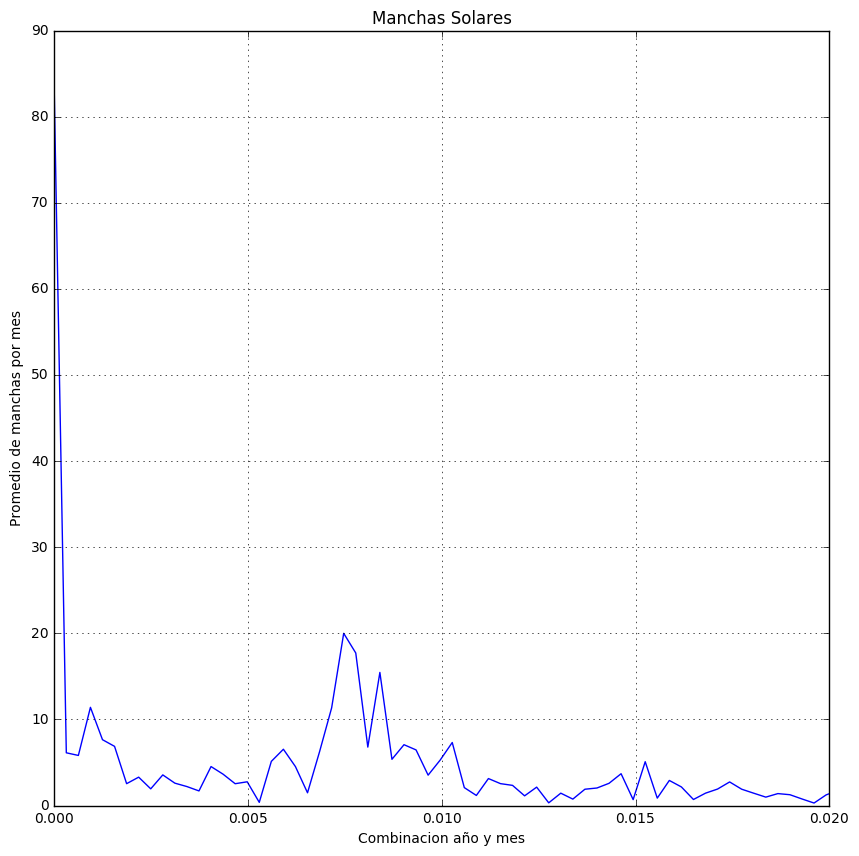
\includegraphics[scale=0.5]{Fouriermanchas.png}
\end{center}

\subsection{Obtención de frecuencias}
\noindent
En la gráfica podemos apreciar una numerosa cantidad de amplitudes, sin embargo, no todas ellas son de nuestro interés, puesto que podemos observar que solo 5 amplitudes son mayores a 10, siendo estos los siguientes:

\begin{center}
\begin{tabular}{|c|c|}
\hline
Dato  & Amplitud \\ \hline
3  &11.39959181\\ \hline
23  &11.33907605\\ \hline
24  &19.9936166\\ \hline
25  &17.709916\\ \hline
27 &15.45401894\\ \hline
\end{tabular}
\end{center}

\noindent
Con la amplitud podemos ayudarnos en ubicar su frecuencia respectiva con el siguiente comando:
\begin{equation*}
Frecuencia =  xf[int(N/2 +1]
\end{equation*}

\noindent
Gracias a ese comando, nos da el punto en la gráfica del eje X en el que se encuentra, dicho eje se trata de las frecuencias por lo que tenemos sus respectivas frecuencias, siendo el de cada uno el siguiente:
\begin{center}
\begin{tabular}{|c|c|c|}
\hline
Dato & Frecuencia & Amplitud \\ \hline
3 & 0.00093370681605975728 &11.39959181\\ \hline
23 & 0.0071584189231248055 &11.33907605\\ \hline
24 &0.0074696545284780582 &19.9936166\\ \hline
25 &0.007780890133831311 &17.709916\\ \hline
27 &0.0084033613445378148 &15.45401894\\ \hline
\end{tabular}
\end{center}

%-------------------------------
\section{Segundo punto}
\noindent
Se encuentran 5 principales, pero podemos nombrar a 2 de ellos que son los más sobresalientes, se muestran como:
\begin{center}
\begin{tabular}{|c|c|c|}
\hline
Dato & Frecuencia & Amplitud \\ \hline
24 &0.0074696545284780582 &19.9936166\\ \hline
27 &0.0084033613445378148 &15.45401894\\ \hline
\end{tabular}
\end{center}

\noindent
Estos son nuestros 2 valores de amplitud más altos. Puesto que son los dos que superan en mayor medida el promedio de 10, con el que al acompañarlo con nuestro dato número 22, se sumaron para poder encontrar un promedio a la frecuencia y se aprovechó para encontrar un valor promedio al periodo:

\begin{equation*}
Frecuencia_{promedio} = 0.0071584189231248055
\end{equation*}

\begin{equation*}
Periodo_{promedio}=11.641304347826088
\end{equation*}

\subsection{Codigo}
\noindent
Frecuencia

$J=(T_{S8}+T_{S9} +T_{S10})/3$\\
J
\\[0.05cm]
\noindent
Periodo

K=1/(J*12)\\
K
%-------------------------------
\section{Tercer punto}
\noindent
Como ya se dijo, se encuentran varias amplitudes que muestran algo de significado, si buscamos los que son mayores a 5 pues pueden verse en la gráfica que se mostró anteriormente, podemos ver que aumentan a un total de 19:
\begin{center}
\begin{tabular}{|c|c|c|}
\hline
Dato & Frecuencia & Amplitud \\ \hline
1 & 0.00031123560535325243 &6.1202308 \\ \hline  
2 &0.00062247121070650485 &5.81322464\\ \hline
3 & 0.00093370681605975728 &11.39959181\\ \hline
4 &0.0012449424214130097 &7.64140607\\ \hline
5 &0.001556178026766262 &6.86795256\\ \hline
18 & 0.0056022408963585435 &5.12470451\\ \hline
19 &0.0059134765017117962 &6.53244749\\ \hline
22 &0.0068471833177715536 &6.2536874\\ \hline
23 & 0.0071584189231248055 &11.33907605\\ \hline
24 &0.0074696545284780582 &19.9936166\\ \hline
25 &0.007780890133831311 &17.709916\\ \hline
26 &0.0080921257391845629 &6.7814543\\ \hline
27 &0.0084033613445378148 &15.45401894\\ \hline
28 &0.0087145969498910684 &5.3662003\\ \hline 
29 &0.0090258325552443203 &7.06077096\\ \hline
30 &0.0093370681605975722 &6.45420329\\ \hline
32 & 0.0099595393713040777 &5.27672092\\ \hline
33 &0.01027077497665733 &7.31412295\\ \hline
49 &0.015250544662309368 &5.08635154 \\ \hline
\end{tabular}
\end{center}

\subsection{Codigo}
\noindent
A=np.absolute(yf)/N\\
A[A[:,]>5]\\
np.where(A[:,]>5)
\\[0.5cm]
\noindent
La obtención de las frecuencias fue utilizando el mismo código del segundo punto.
%------------------------------

\section{Cuarto punto}
\noindent
Se toma el valor en cero como un promedio del ciclo completo, en nuestro caso la amplitud de nuestro cero es de 82.9236 aproximadamente. Con esto como un valor promedio podemos proceder a tener una sumatoria de senos y cosenos, dicha sumatoria nos da como resultado una probabilidad donde puede haber un numero de manchas solares en cierto rango de valores. No se tiene exactamente un método de predicción sobre las manchas solares como para decir de forma segura cuándo ocurrirá una mancha solar, por eso todo se deja basándose en probabilidades utilizando un promedio del ciclo y un rango de valores en el que quizás ocurra o quizás no ocurra dicho evento. Solo se puede decir que quizás ocurra una mancha dada la proximidad que se puede obtener, pero nunca habrá un método seguro, al menos no en este momento que se realizó esta evaluación con las fuentes de información dadas en las mismas instrucciones de la evaluación.
\end{document}
